%!TEX root = ../main.tex

\section*{Methods}

  The flowchart describing the workflow of the \ac{mind} pipeline is as shown in Figure \ref{fig:mind_pipeline}.
  The pipeline seamlessly integrates many publicly available tools as well as custom Python modules and scripts to extract co-occurrence associations from 16S sequence data.
  The input to the pipeline by default is the raw 16S rRNA sequence data, but it can be configured to use processed sequences, \ac{otu} tables or other types of intermediate data as well.
  The final output of the pipeline is the inferred network of co-occurrence associations among the microbes present in the samples.
  In order to determine the best combination of tools for the pipeline, we examine the effects of each tool on the final co-occurrence network.
  We can then estimate the variance contributed by each step in the pipeline to the total variance present across the networks.
  We propose to use mock synthetic data simulated using an Illumina read-simulator \cite{Escalona2016} and a mock community data-set \cite{Bokulich2016} as standards for comparing the counts matrices and the assigned taxonomies.
  We will then use a voting method to obtain a co-occurrence network that has links predicted by multiple network inference methods.

  Some key features of the pipeline include modularity, flexibility and ease-of-use.
  The entire pipeline consists of modules which can be modified, reordered or replaced appropriately using a simple configuration script.
  The only thing needed to process data through the pipeline is the package itself and a configuration script that lists the steps to be performed, along with the parameters to be used (optional).
  The pipeline allows for automatic parallelization of all possible processes, both within and across samples.
  The entire pipeline has been containerized into a Docker \cite{Merkel1994} image for easy deployment and setup.
  The main components of the pipeline are detailed in the following section.

  \begin{figure}[h]
    \centering
    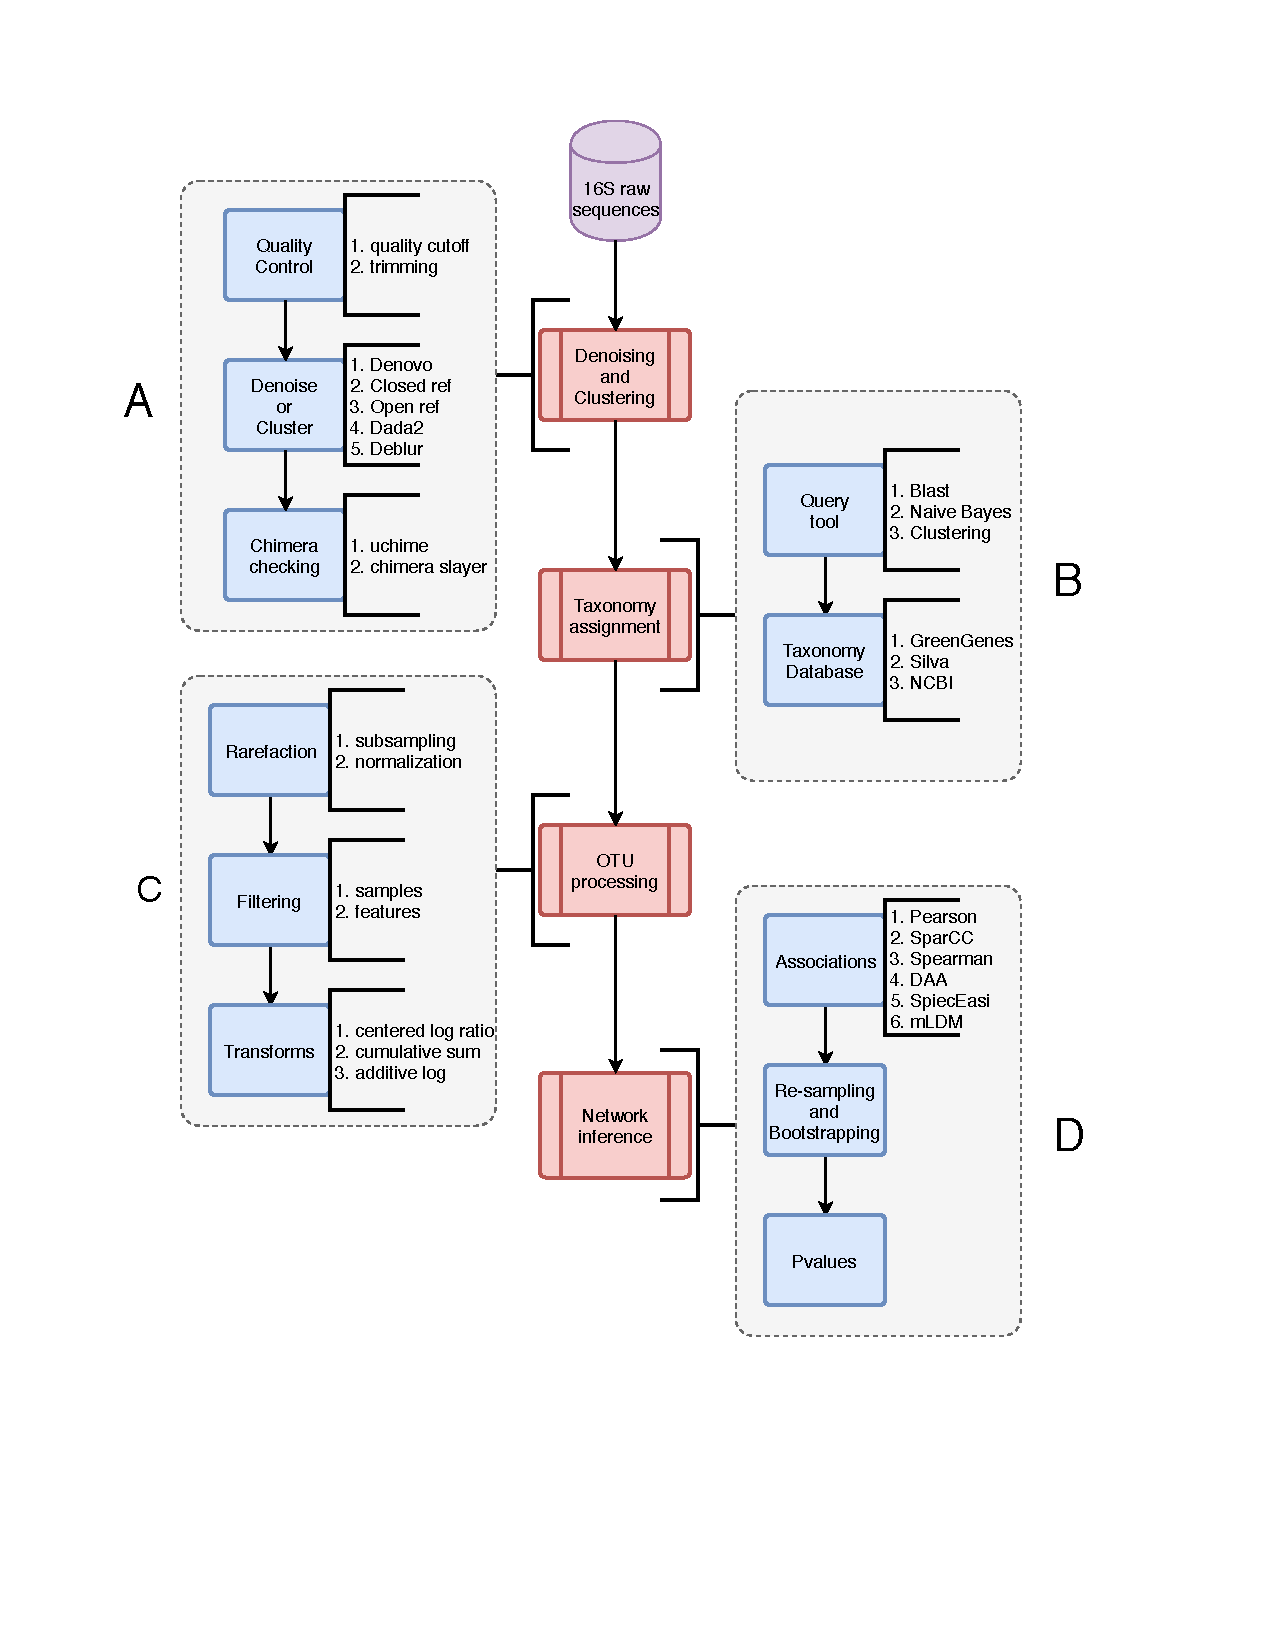
\includegraphics[width=0.7\textwidth]{mind_pipeline.pdf}
    \caption{
      \textbf{The workflow of the microbial co-occurrence analysis pipeline}.
        The processes can be grouped into four major components - denoising and clustering (A), taxonomy assignment (B), \ac{otu}/\ac{esv} processing (C), and network inference (D).
        Each of these incorporate several processes, each of which in turn have several alternate algorithms for the same task (as indicated by the text to the right of the blue boxes).
    }
    \label{fig:mind_pipeline}
  \end{figure}

  \subsubsection*{Denoising and Clustering}
    \vspace{-5mm}
    This module deals with processing the raw 16S sequence data into \ac{otu} or \ac{esv} count tables.
    It incorporates three processes: quality control, denoise/cluster and chimera checking.
    \begin{itemize}
      \item The quality control process handles the demultiplexing and quality control steps such as trimming adapters and trimming low-quality nucleotide stretches from the sequences.
      \item The denoise/cluster process handles the conversion of the demultiplexed, trimmed sequences into \ac{otu} or \ac{esv} count tables \footnote{Some methods perform clustering and taxonomy assignment in the same step}.
      \item The chimera checking process handles the removal of chimeric sequences created during the \ac{pcr} step.
    \end{itemize}
    The output of this module is a counts matrix that describes the number of reads of a particular \ac{otu} or \ac{esv} (rows of the matrix) present in each sample (columns of the matrix). The pipeline incorporates \ac{qiime1} \cite{Caporaso2010}, \ac{qiime2}, \ac{dada2} \cite{Callahan2016} and Deblur \cite{Amir2017} tools in this module.

  \subsubsection*{Taxonomy Assignment}
    \vspace{-5mm}
    This module deals with assigning taxonomies to either the representative sequences of the \ac{otu}s or directly to the \ac{esv}s.
    In order to assign taxonomies to a particular sequence we need two things: a query tool and a taxonomy database.
    The taxonomy database is a collection of 16S sequences of known organisms.
    The query tool allows one to compare a sequence of interest to all the sequences in the database to find the best match.
    The pipeline already incorporates \ac{gg} \cite{DeSantis2006}, SILVA \cite{Quast2012} and will soon include the \ac{ncbi} \cite{Sayers2009} as well.

  \subsubsection*{OTU and ESV Processing}
    \vspace{-5mm}
    This module deals with normalization, filtering and applying transformations on the \ac{otu} or \ac{esv} counts matrix.
    \begin{itemize}
      \item Rarefaction is a normalization technique used to overcome the bias that might arise due to variable sampling depth \footnote{The total number of reads obtained from a particular sample} in different samples. This is commonly performed either by sub-sampling or by normalization of the matrix to the lowest sampling depth.
      \item Filtering is usually performed to remove samples or features from the count matrix that are sparse.
      \item Transformations are performed in order to correct for and overcome the compositional bias that is inherent in a counts matrix.
    \end{itemize}

  \subsubsection*{Network Inference}
    \vspace{-5mm}
    This module deals with the inference of co-occurrence associations from the \ac{otu} or \ac{otu} counts matrix. These associations can be represented as a network.
    \begin{itemize}
      \item Associations can either be correlations or direct associations.
      \item Significance of these associations is determined by re-sampling, bootstrapping and calculating pvalues.
    \end{itemize}
    The pipeline incorporates \ac{sparcc} \cite{Friedman2012} and \ac{spieceasi} \cite{Kurtz2015} and will soon include \ac{mldm} \cite{Yang2017} and \ac{daa} \cite{Menon2018}.

  \subsubsection*{MIND Data Visualizer}

    In addition to the web application and pipeline, we have also developed a tool that facilitates easy visualization and exploration of the data generated by the \ac{mind} pipeline.
    This tool is a Python package and is built using dash \cite{dash}.
    It aids in the analysis of the effects of different processing methods on the generated counts matrix or network.
    It takes in as input the results of a pipeline run and allows one to visualize various properties of intermediate \ac{otu} or \ac{esv} tables and final association networks.
    This tool makes it easy and straightforward to compare different methods and combinations of methods in the 16S data analysis workflow.

    The visualization tool currently supports:
    \begin{itemize}
      \item Filtering and aggregating data from multiple sources (data-sets)
      \item Comparing properties of the generated counts matrices and networks across different methods
      \item Visualization of these properties
    \end{itemize}
